%\documentclass[11pt]{beamer}
\documentclass[11pt,handout,aspectratio=1610]{beamer}

\usepackage[utf8]{inputenc}
\usepackage[T1]{fontenc}
\usepackage[spanish]{babel}
\usepackage{latexsym} 
\usepackage{amsmath}
\usepackage{amsfonts}
\usepackage{amssymb}
\usepackage{esint}
\usepackage{array}
\usepackage{multirow}
\usepackage{xcolor}
\usepackage{graphicx}
\usepackage{tikz}
\usepackage{tikz-3dplot}
\usetikzlibrary{babel}
\usetikzlibrary{calc,patterns,decorations.pathmorphing,decorations.markings}
\usepackage{xcolor}
\usepackage{epstopdf}
\usepackage[nointegrals]{wasysym}
\usepackage{hyperref}
\usepackage{cancel}

\usetheme{Berkeley}
\usecolortheme{seahorse}
\uselanguage{Spanish}

\newcommand{\sgn}{\mathop{\text{sgn}}}
\newcommand{\diff}[0]{\text{d}}
\newcommand{\fdiff}[2]{\dfrac{\text{d} #1}{\text{d} #2}}
\newcommand{\pdiff}[2]{\frac{\partial #1}{\partial #2}}
\newcommand{\fddiff}[2]{\frac{\text{d^2} #1}{\text{d} #2^2}}
\newcommand{\degr}[0]{^{\circ}}
\newcommand{\chel}[4]{^{#1}_{#2}\text{#3}^{#4}}
\newcommand{\valmed}[1]{\left\langle #1 \right\rangle}
\newcommand{\E}[1]{\times 10^{#1}}
%\renewcommand{\vec}[1]{\text{\textbf{#1}}}
\newcommand{\ver}[1]{\hat{\vec{#1}}}
\newcommand{\vecg}[1]{\boldsymbol{#1}}
\newcommand{\iu}{\text{i}}
\newcommand{\norm}[1]{\left\lVert #1 \right\rVert }
\newcommand{\abs}[1]{\left\vert #1 \right\vert}
\newcommand{\tens}[1]{\mathbb{#1}}
\newcommand{\rr}{\mathbb{R}}
\newcommand{\logoUNAHUR}{
\includegraphics[scale=0.15]{/home/shluna/Proyectos/Clases_Fisica_III/imgs/logo-universidad-nacional-de-hurlingham_preview_rev_1.png}}
\newcommand{\vs}{\vspace{0.3cm}}
\newcommand{\un}[1]{\text{#1}}
\renewcommand{\arraystretch}{1.2}

\title{Sistemas de partículas y cuerpo rígido}
\subtitle{Unidad 2}
\author{Física III}
\institute{Instituto de Tecnología e Ingeniería \\ \vspace{0.25cm} Universidad Nacional de Hurlingham}
\date{Segunda parte}
\logo{\logoUNAHUR}

\AtBeginSection[]{
  \begin{frame}
  \vfill
  \centering
  \begin{beamercolorbox}[sep=8pt,center,shadow=true,rounded=true]{title}
    \usebeamerfont{title}\insertsectionhead\par%
  \end{beamercolorbox}
  \vfill
  \end{frame}
}

\tdplotsetmaincoords{70}{110}

\begin{document}

\renewcommand{\tablename}{Tabla}

\frame{\titlepage}

\begin{frame}{En esta clase veremos:}
    \tableofcontents
\end{frame}

\section{Concepto de cuerpo rígido}

\begin{frame}{Cuerpo rígido}

\begin{block}{Definición}
    Un cuerpo rígido es un sistema de partículas en el que la distancia entre cada par de partículas que lo conforman es constante.
\end{block}

\begin{columns}
    \begin{column}{0.5\textwidth}
        \begin{figure}
            \centering
            \begin{tikzpicture}    
                \pgfmathsetseed{3}
                \draw[fill=gray!40] plot [smooth cycle, samples=8,domain={1:8}](\x*360/8+5*rnd:0.8cm+1.5cm*rnd) node at (0,0) {};
                \draw[thick,-latex] (-0.5,-1) -- node[anchor=south east]{\scriptsize $\vec{r}_i$} (45:0.8);
                \fill[black] (-0.5,-1) circle (0.3mm) node[anchor=north]{\scriptsize $O$};
                \fill[black] (45:0.8) circle (0.3mm) node[anchor=west]{\scriptsize $i$};
                \draw[thick,-latex] (-0.5,-1) -- node[anchor=north west]{\scriptsize $\vec{r}_j$} (-30:0.9);
                \fill[black] (-30:0.9) circle (0.3mm) node[anchor=west]{\scriptsize $j$};
                \draw[thick,-latex] (45:0.8) -- node[anchor=west]{\scriptsize $\vec{r}_j - \vec{r}_i$} (-30:0.9);
            \end{tikzpicture}
        \end{figure}
    \end{column}
    \begin{column}{0.5\textwidth}
        La distancia entre cada par de partículas $i$ y $j$ no cambia en el tiempo. Esto es: $$\norm{\vec{r}_j - \vec{r}_i} = \text{constante}$$ En otras palabras, un cuerpo rígido es un sistema de partículas \emph{indeformable}.
    \end{column}
\end{columns}

\vs

Si bien es una idealización, el concepto de cuerpo rígido es muy útil y, en muchos casos, es una buena aproximación a la realidad.

\end{frame}

\section{Rotación de un rígido alrededor de un eje fijo}

\begin{frame}{Rotación de un rígido alrededor de un eje fijo}

    Vamos a estudiar el movimiento de sólidos rígidos alrededor de un eje fijo. \pause

\begin{columns}
    \begin{column}{0.3\textwidth}
        \begin{figure}
            \centering
            \begin{tikzpicture}[scale=1.2] 
                \pgfmathsetseed{3}
                \draw[fill=gray!40] plot [smooth cycle, samples=8,domain={1:8}](\x*360/8+5*rnd:0.5cm+1cm*rnd) node at (0,0) {};
                \draw[thick,-latex] (0,0) -- node[anchor=south east]{\scriptsize $\vec{r}_i$} (45:0.8);
                \fill[black] (0,0) circle (0.3mm);
                \fill[black] (45:0.8) circle (0.3mm) node[anchor=west]{\scriptsize $i$};
                \draw[dashed] (0,0) circle (0.8);
            \end{tikzpicture}
        \end{figure}
    \end{column} \pause
    \begin{column}{0.7\textwidth}
        \begin{itemize}
            \item La velocidad angular de todas las partículas es la misma $\vec{\omega}_1 = \vec{\omega}_2 = \ldots = \vec{\omega}_i = \ldots = \vec{\omega}_N$. \pause 
            \item Por lo tanto, podemos hablar de la \emph{velocidad angular del cuerpo rígido} ($\vec{\omega}$). \pause
            \item Lo mismo ocurre con la aceleración angular ($\vec{\alpha}$).
        \end{itemize}
    \end{column}
\end{columns}

\end{frame}

\begin{frame}{Rotación de un rígido alrededor de un eje fijo}

    El estado dinámico de una masa puntual se especifica indicando su posición y su velocidad.

    \vspace{11pt}

    De forma análoga, el estado dinámico de un cuerpo rígido se especifica unívocamente en cada instante de tiempo indicando su orientación y su velocidad angular.

    \vspace{11pt}

    Si asumimos que el cuerpo rígido rota con velocidad angular constante, entonces la posición de cada partícula se determina conociendo su distancia al eje ($r_i$) y el ángulo ($\theta_i$) que forma el vector de posición con el semieje de los $x$ positivos, por ejemplo, donde $$\theta_i (t) = \omega \left(t - t_0\right) + \theta_{0,i}$$
    
\end{frame}

\begin{frame}{Rotación de un rígido alrededor de un eje fijo}

    Ahora bien, al cabo de un intervalo de tiempo arbitrario, el desplazamiento angular será el mismo para todos los puntos que conforman el cuerpo rígido.

    \vspace{11pt}

    En este sentido, la orientación del cuerpo rígido queda especificado por el ángulo que forma el vector de posición de una cualquiera de las partículas antes mencionadas. 
    
    \vspace{11pt}

    Por lo tanto, podemos identificar dicho ángulo como aquél que da la orientación del cuerpo rígido en un instante de tiempo determinado.

\end{frame}

\begin{frame}{Rotación de un rígido alrededor de un eje fijo}

    Así, en el caso aquí considerado, se puede afirmar que la \emph{orientación} del cuerpo rígido queda determinada por la expresión: $$\theta (t) = \omega \left(t - t_0\right) + \theta_0$$ donde ahora $\theta$ es el ángulo que forma la recta que une el punto de intersección del eje alrededor del cual gira el cuerpo rígido con otro punto arbitrario del mismo, que se toma como referencia.

    \begin{center}
        \begin{tikzpicture}[scale=1.2] 
            \pgfmathsetseed{3}
            \draw[fill=gray!40] plot [smooth cycle, samples=8,domain={1:8}](\x*360/8+5*rnd:0.5cm+1cm*rnd) node at (0,0) {};
            \draw[-latex] (-2,0) -- (2,0) node[anchor=north]{\scriptsize$x$};
            \draw (0,0) -- (45:1.5);
            \draw (0.25,0) arc (0:45:0.25);
            \node[anchor=south west] at (0.25,0) {\scriptsize $\theta$};
            \draw[thick,-latex] (0,0) -- node[anchor=south east]{\scriptsize $\vec{r}_i$} (45:0.8);
            \fill[black] (0,0) circle (0.3mm);
            \fill[black] (45:0.8) circle (0.3mm) node[anchor=west]{\scriptsize $i$};
            \draw[dashed] (0,0) circle (0.8);
        \end{tikzpicture}
    \end{center}

\end{frame}

\section{Momento angular de un cuerpo rígido}

\begin{frame}{Momento angular de un cuerpo rígido}

    El momento angular de cada partícula del cuerpo rígido que se mueve en una trayectoria circular es: $$\vec{L}_i = I_i \, \vec{\omega}_i = m_i \, r_i^2 \, \vec{\omega}_i$$
    
    \vs

    Luego, el momento angular total de un sistema de partículas es la suma de los momentos angulares de cada partícula: $$\vec{L} = \sum_{i=1}^N \vec{L}_i = \sum_{i=1}^N m_i \, r_i^2 \, \vec{\omega}_i$$
    
\end{frame}
    
\begin{frame}{Momento angular de un cuerpo rígido}

    Nuevamente, como la velocidad angular es la misma para todas las partículas que componen el cuerpo rígido, $\vec{\omega}_i = \vec{\omega}$, entonces: $$ \vec{L} = \left(\sum_{i=1}^N m_i \, r_i^2\right) \vec{\omega} $$ En consecuencia:
    \begin{equation*}
        \boxed{\vec{L} =  I \, \vec{\omega},}
    \end{equation*} donde ahora $I$ es el momento de inercia del cuerpo rígido: $$ I = \sum_{i=1}^N m_i \, r_i^2 = \sum_{i=1}^N I_i $$ donde $I_i = m_i \, r_i^2$ es el momento de inercia de cada partícula que conforma el cuerpo rígido.
    
\end{frame}

\section{Energía cinética de un cuerpo rígido}

\begin{frame}{Energía cinética de un cuerpo rígido}

La energía cinética de un sistema de partículas es $$E_\text{c} = \sum_{i=1}^N \frac{1}{2} m_i \, v_i^2$$ \pause En virtud de que todas las partículas que conforman el cuerpo rígido describen una circunferencia alrededor del punto por donde pasa el eje alrededor del cual gira el cuerpo rígido, entonces $v_i = r_i \, \omega_i$, y por lo tanto: $$E_\text{c} = \sum_{i=1}^N \frac{1}{2} m_i \left(r_i \, \omega_i\right)^2 = \sum_{i=1}^N \frac{1}{2} m_i \, r_i^2 \, \omega_i^2$$

\end{frame}

\begin{frame}{Energía cinética de un cuerpo rígido}

Como la velocidad angular de todas las partículas es la misma, $\omega_i = \omega$: $$E_\text{c} = \frac{1}{2} \left(\sum_{i=1}^N m_i \, r_i^2\right) \omega^2$$ donde $$ I = \sum_{i=1}^N m_i \, r_i^2$$ es el \emph{momento de inercia} del cuerpo rígido. Así, llegamos a la expresión matemática de la
    
\begin{block}{Energía cinética de un cuerpo rígido}
    $$E_\text{cr} = \frac{1}{2} I \, \omega^2$$
\end{block} 

\end{frame}

\section{Momento de inercia}

\begin{frame}{Momento de inercia}

    La expresión $$I = \sum_{i=1}^N m_i \, r_i^2$$ permite calcular el momento de inercia para un conjunto de partículas. Para una sola partícula: $I = m \, r^2$.

    \vs

    Para un cuerpo sólido considerado como un medio continuo, la suma se transforma en una integral: $$ I = \int\limits_\text{cuerpo} r^2 \, \text{d}m$$ La integral se puede interpretar como la suma de infinitos elementos diferenciales de masa $\text{d}m$ multiplicados por la distancia de cada uno al eje alrededor del cual giran.

\end{frame}

\begin{frame}{Momento de inercia}

    Cada elemento de masa puede expresarse como $\diff{m} = \rho (\vec{r}) \, \diff{V}$ donde $\vec{r}$ es el vector de posición del $\diff{m}$. Reemplazando en la integral, se obtiene: $$ I = \int\limits_\text{cuerpo} \rho (\vec{r}) \, r^2 \, \text{d}V$$ Si se asume que la distribución de masa del cuerpo es uniforme, se tiene que $\rho (\vec{r}) = \rho$ y, en consecuencia: $$ I = \int\limits_\text{cuerpo} \rho (\vec{r}) \, r^2 \, \text{d}V = \rho \int\limits_\text{cuerpo} r^2 \, \text{d}V$$ Así se pueden obtener expresiones analíticas para sólidos que tengan formas geométricas en particular.

    
\end{frame}

\begin{frame}{Momento de inercia}
    
    \begin{figure}
        \centering
        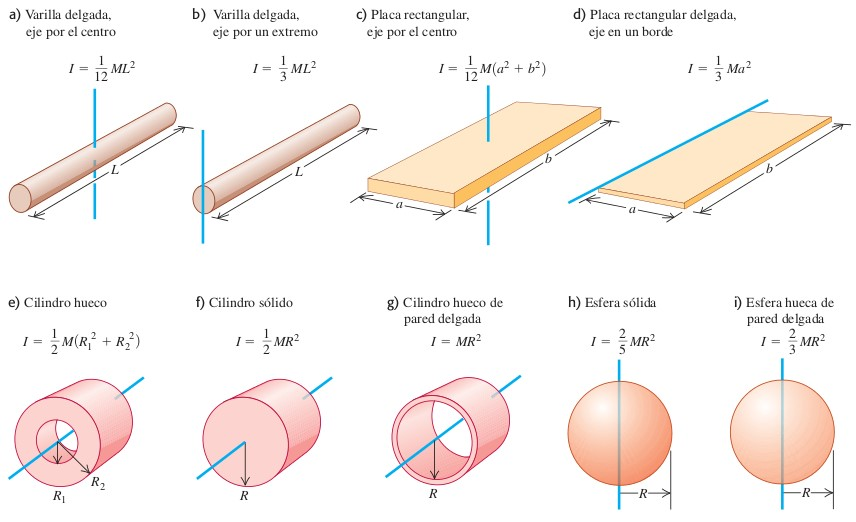
\includegraphics[width=0.9\textwidth]{/home/shluna/Proyectos/Clases_Fisica_III/figs/momentos_de_inercia.jpg}
    \end{figure}

\end{frame}

\begin{frame}{Momento de inercia}
    
    \begin{alertblock}{¡Importante!}
        Como el momento de inercia se puede calcular respecto a un eje arbitrario, se deduce entonces que este \emph{no} es una propiedad intrínseca del cuerpo, tal como su masa. 

        \vspace{11pt}
        
        En otras palabras, el momento de inercia \emph{depende} de dónde se lo mide, en cambio, el valor de la masa de un cuerpo es independiente del sistema de referencia elegido. 
    \end{alertblock}

\end{frame}

\begin{frame}{Radio de giro}

    Independientemente de la forma del cuerpo, \emph{siempre} es posible encontrar una distancia al eje dado a la cual pudiera concentrarse la masa del del cuerpo sin modificar el momento de inercia del mismo respecto al mismo eje. \pause

    \vspace{11pt}

    Esta distancia se conoce como \emph{radio de giro}.

\end{frame}

\begin{frame}{Radio de giro}

    Sea un cuerpo de forma arbitraria de masa total $M$ y sea $I_\text{cuerpo}^{(O)}$ su momento de inercia respecto a un eje que pasa por el punto $O$. \pause Queremos encontrar la distancia $k$ a la cual debería estar un punto cuya masa es $M$ para que produzca el mismo momento de inercia que el cuerpo.

    \begin{columns}
        \begin{column}{0.5\textwidth}
            \begin{figure}
                \centering
                \begin{tikzpicture}    
                    \pgfmathsetseed{3}
                    \draw[fill=gray!40] plot [smooth cycle, samples=8,domain={1:8}](\x*360/8+5*rnd:0.5cm+1cm*rnd) node at (0,0) {};
                    \draw (0,0) -- node[anchor=north west]{\scriptsize $R_\text{giro}$} (30:2.5);
                    \fill[black] (0,0) circle (0.5mm) node[anchor=north]{\scriptsize $O$};
                    \fill[black] (30:2.5) circle (0.5mm) node[anchor=north]{\scriptsize $P$};
                    \node at (270:0.8) {\scriptsize $M$};
                    \node[anchor=south] at (30:2.5) {\scriptsize $M$};
                \end{tikzpicture}
            \end{figure}
        \end{column} \pause
        \begin{column}{0.5\textwidth}
            {\small
            $$I_\text{mp}^{(O)} = M \, R_\text{giro}^2$$ \pause
            $$M \, R_\text{giro}^2 = I_\text{cuerpo}^{(O)}$$ \pause
            $$R_\text{giro} = \sqrt{\frac{I_\text{cuerpo}^{(O)}}{M}}$$
            }
        \end{column}
    \end{columns}

\end{frame}

\begin{frame}{Esto es todo por hoy}

    \begin{center}
        {\huge ¡Muchas gracias!}

        \vs

        Ahora a repasar y practicar.
    \end{center}

\end{frame}

\end{document}

\begin{frame}{}



\end{frame}